\documentclass[master]{thesis-uestc}
% 此处-----------|---的模板类型设置请参照README
\title{大功率宽频带脊波导微波窗研究}{English Title} % 论文题目
\author{方源}{English Name} % 作者姓名
\setdate[submit]{ } % 论文提交日期,可留空
\setdate[oral]{ }  % 答辩日期,可留空
\setdate[confer]{ } % 学位授予日期,可留空
\advisor{\qquad 王建勋\qquad\qquad 教\chinesespace 授}{English name English title}
% \coAdvisor{合作导师姓名\chinesespace 导师职称}{Co advisor English name English title} % 仅专业硕士/博士使用,在扉页/英文首页添加合作导师,不使用请注释
\school{电子科学与工程学院}{School of Electronic Science and Engineering} % 学院信息
\major{电子科学与技术}{Electronic Science and Technology} % 专业信息
\studentnumber{202221020122} % 学号
\ProfessionalDegreeArea{随便学学} % 专业硕士专用:专业学位领域
\ClassificationNumber{TP309.2} % 分类号
\ClassifiedClass{公开} % 密级
\UDCNumber{004.78} % UDC号
\Chairman{xxxxx} % 答辩委员会主席

% 取消注释以下内容,用于禁止文中换行处的英语单词自动截断换行。
% \tolerance=1
% \emergencystretch=\maxdimen
% \hyphenpenalty=10000
% \hbadness=10000

\makeglossaries % 产生缩略词表/符号表专用,不使用时请注释。 注意,之后的acronym,glossaryentry以及相关的引用也请注释。
\newacronym[description=逻辑卷管理器]{lvm}{LVM}{Logical Volume Manager} % 定义缩略词:以本项为例,逻辑卷管理器为中文名称;lvm用于文内引用;LVM为显示的应为缩略语或符号;Logical Volume Manager为显示的英文全称/描述。
\newglossaryentry{tree}{name={tree}, description={trees are the better humans}}  % 定义符号:以本项为例,name={tree}为符号名称;tree用于文内引用; description={trees are the better humans}为显示的描述。页码自动添加。

\begin{document}

\makecover % 封面+中英文扉页
\originalitydeclaration % 原创新声明
% \signatureofdeclaration{signature.pdf} % 用于添加扫描版签字后的原创新声明(使用时取消注释本行,并注释掉上一行)
% 中文摘要
\begin{chineseabstract}

    \chinesekeyword{xxx,xxx,xxx} % 中文关键词
\end{chineseabstract}
% 英文摘要
\begin{englishabstract}

    \englishkeyword{xxx, xxx, xxx} % 英文关键词
\end{englishabstract}

\thesistableofcontents % 目录
\thesisfigurelist % 图目录,仅在需要时添加,一般情况下请注释
\thesistablelist % 表目录,仅在需要时添加,一般情况下请注释
% \glsaddall % 默认仅显示被正文引用的项,取消注释以显示所有已定义的缩略词/符号
\thesisglossarylist % 缩略词表,仅在需要时添加,一般情况下请注释
\thesissymbollist % 符号表,仅在需要时添加,一般情况下请注释

% 正文内容


\chapter{绪\hspace{6pt}论}
\section{生活中的微波真空管器件}
\section{真空管的微波窗}
\section{真空管中的宽带宽需求}
\section{国内外研究现状}

\section{论文结构与安排}
\chapter{微波窗的理论研究}
\section{经典微波窗的理论分析}
随着时代的发展,微波窗的这种累也趋于多种多样,在理论研究方面比较完备的微波窗是盒型窗与同轴窗,这两种窗的结构较为简单便于使用场匹配或者等效电路法进行研究。由于对这两种窗的结构理论研究有助于后续的窗片设计,故现在此对这两种窗的基本理论进行相应的论述。
\subsection{盒型窗的理论研究}\label{subsec:PillBoxTheory}
常见的盒型窗的主要是由负责进行传输的矩形波导、一个薄圆片形状的介质窗片以及窗片两侧的匹配圆柱波导组成,这其中蕴含了的电磁场边界条件的不连续性,可以使用等效电路法来进行研究。此时将盒型窗的两侧波导以及窗片两侧的空气圆柱部分等效为波导传输线,将较为薄的窗片、矩形波导与圆柱形波导之间的不连续性和窗片与圆柱形波导之间的不连续性等效为电纳。并以此等效思路为基础构建微波窗的等效电路,进而求解电路的频率响应。

常规的盒型窗的矩形波导的工作频率为$TE_{10}$模式,其中的圆形窗片的主要工作模式为$TE_{11}$模式,这两种模式均为波导的基模。当矩形波导和圆波导进行直接耦合的时候根据文章\citing{Bharathi2015DESIGNAD, marcuvitz_waveguide_1986_rec_cylinder}的研究表明,此时会出现不连续性,在等效电路中相当于引入了一个等效电纳$B_{T}$,此时根据式子\ref{eq:B_T}这个等效电纳可以被表示为:
\begin{equation}\label{eq:B_T}
    B_{T}=\frac{b}{\lambda_{g r}}\left\{2 \ln \left(\frac{D^{2}-b^{2}}{4 b D}\right)+\left(\frac{b}{D}+\frac{D}{b}\right) \ln \left(\frac{D+b}{D-b}\right)+2 \sum_{n=1}^{\infty} \frac{\sin ^{2} n \phi}{n^{3} \phi^{2}} \delta_{2 n}\right\}
\end{equation}
此时式子中的$D$为圆形波导的直径,$a$和$b$分别为矩形波导的长边长度和短边长度,$\beta$为矩形波导的传播常数,$\lambda_{g r}$为矩形波导的工作波长,$\lambda_{g c}$为圆形波导的工作波长,$t$为圆柱形介质窗片的厚度,$\omega$为微波窗的角工作频率,$c$为真空的光速,$\lambda$为自由空间中的波长。

为了便于封装焊接,窗片的直径最好等于矩形波导的对角线长度,此时根据勾股定理我们可以得到窗片直径$D$和矩形波导长短边之间的关系$D=\sqrt{a^2+b^2} $。关于计算式最后的求和式中的$\delta_{2n}$和$\phi$的计算方法可以被表示为式子\ref{eq:delta_phi}中的\ref{eq:delta}到\ref{eq:phi}所示:
\begin{subequations}\label{eq:delta_phi}
\begin{align}
    \delta_{2 n} &= \frac{1}{\sqrt{1-\left(\frac{\beta \mathrm{D}}{2 \pi n}\right)^{2}}}-1 \label{eq:delta}\\
    \beta &= \frac{2 \pi}{\lambda_{gr}} \label{eq:beta}\\
    \phi &= \frac{\pi b}{D} \label{eq:phi}
\end{align}
\end{subequations}
根据之前分析的盒型窗中存在的三个不连续性边界条件,可以将原先的盒型窗等效为如--所示的等效电路,在这个等效电路中,$Z_{cir}$是真空填充的圆柱形波导的特征阻抗,$Z_{rec}$是矩形波导的特征阻抗,$B_{d}$是圆形窗片引入不连续性所等效的归一化电纳,$B_{T}$是由于矩形波导与圆柱形波导之间的不连续性引入的归一化电纳。

根据微波网络理论,这个两端口的等效电路可以被表示为一个如\ref{eq:ABCD}所示的$ABCD$矩阵,其中$k=Z_{cir}/Z_{rec}$,是真空填充的圆柱形的特征阻抗按照矩形波导的特征阻抗所归一化的特征阻抗比值;$\gamma=\frac{2 \pi}{\lambda_{gc}}$是真空填充的圆柱形波导的传播常数,$l$是介质窗片两侧的真空填充的圆柱形波导的纵向长度。
\begin{equation}\label{eq:ABCD}
    \begin{split}
        \begin{bmatrix}
            A & B \\
            C & D
        \end{bmatrix} 
        & = 
        \begin{bmatrix}
            \sqrt{k} & 0 \\
            jB_{T}\sqrt{k} & 1/\sqrt{k}
        \end{bmatrix}
        \begin{bmatrix}
            \cos{\gamma l} & j\sin{\gamma l} \\
            j\sin{\gamma l} & \cos{\gamma l}
        \end{bmatrix}
        \begin{bmatrix}
            1 & 0 \\
            jB_{d} & 1
        \end{bmatrix} \\
        & \quad \times 
        \begin{bmatrix}
            \cos{\gamma l} & j\sin{\gamma l} \\
            j\sin{\gamma l} & \cos{\gamma l}
        \end{bmatrix}
        \begin{bmatrix}
            1/\sqrt{k} & 0 \\
            jB_{T}\sqrt{k} & \sqrt{k}
        \end{bmatrix}
    \end{split}
\end{equation}

由于此时的窗片的厚度相比于使用窗片介质填充的圆柱形波导的工作波长来说太短,其引入的不连续性可以被等效为电纳$B_{d}$,详细的计算式是式\ref{eq:B_d},其中$t$为窗片的厚度,$\varepsilon_d$为窗片的相对介电常数:
\begin{equation}\label{eq:B_d}
    B_{d} = t (\varepsilon_d - 1) \left( \frac{\omega}{c} \right) \left( \frac{\lambda_{gc}}{\lambda} \right)
\end{equation}

此时,假设盒型窗的输入功率为$P_{1}$,通过盒型窗之后输出功率为$P_{2}$,根据S参数以及$ABCD$矩阵的定义,我们可以得到$P_{2}$与$P_{1}$的比值为式子\ref{eq:P2P1}:
\begin{equation}\label{eq:P2P1}
    \frac{P_{2}}{P_{1}} = \frac{1}{1+\frac{1}{4} (B-C)^2}
\end{equation}
那么根据能量守恒定律,假设窗片不存在损耗,那么其反射系数$|\Gamma|$可以被表示为式子\ref{eq:Gamma}:
\begin{equation}\label{eq:Gamma}
    |\Gamma| = \left| 1 - \left( \frac{P_{2}}{P_{1}} \right) \right|^{\frac{1}{2}}
\end{equation}
假设窗片完全传输,那么此时的$P_{2}=P_{1}$,进而根据式子\ref{eq:P2P1}可以推理出来$ABCD$矩阵中的$B=C$。为了获得一个可以确定盒型窗的几何参数的进行求解的方程,有必要进行几点假设:
\begin{enumerate}
    \item 此时的真空填充的圆柱形波导的长度$l$可以较为任意的进行选取,注意是较为任意的选取不是完全任意的选取,因为如果真空填充的圆柱形波导的长度过短,会导致圆柱形波导部分无法被等效为一段传输线,进而导致原先的等效电路模型失效。
    \item 窗片的材料已经确定,也就是窗片的相对介电常数$\varepsilon_{d}$是一定的。
    \item 要求匹配到的频点$f$为已经确定的值,也就是$\lambda$、$\lambda_{gc}$和$\lambda_{gr}$是已经确定的。
\end{enumerate}


现在我们将原先式子\ref{eq:ABCD}的几个矩阵元素完全相乘,可以得到计算式\ref{eq:ABCD_solved},式子中\ref{eq:A}到\ref{eq:D}为计算式\ref{eq:ABCD}中$ABCD$矩阵的四个元素:
\begin{subequations}\label{eq:ABCD_solved}
    \begin{align}
        A &= \frac{1}{2} \big[-(B_d + 2 B_T k) \sin(2\gamma l) + (2 - B_d B_T k)\cos(2\gamma l) + B_d B_T k \big] \label{eq:A} \\
        B &= -i k \sin(\gamma l) (B_d \sin(\gamma l) - 2 \cos(\gamma l)) \label{eq:B} \\
        C &= \frac{i (\cos(\gamma l) - B_T k \sin(\gamma l)) \big[(2 - B_d B_T k)\sin(\gamma l) + (B_d + 2 B_T k)\cos(\gamma l)\big]}{k} \label{eq:C} \\
        D &= \frac{1}{2} \big[-(B_d + 2 B_T k) \sin(2\gamma l) + (2 - B_d B_T k)\cos(2\gamma l) + B_d B_T k \big] \label{eq:D}
    \end{align}
\end{subequations}

注意到推演结果中$A$元素与$D$元素相等,这与微波网络中的理论描述相符。此时为了满足$ABCD$矩阵的$B$与$C$元素相等,我们可以将这两个元素进行作差处理,如果相等的话那么可以得到$B-C=0$,进一步的,可以得到如下关于作差后的表达式\ref{eq:B-C-simplify1}:

\begin{equation}\label{eq:B-C-simplify1}
    \begin{split}
        B - C = & -\frac{i}{2k} \Bigg( \Big[-B_{d}(B_{T}^2 + 1)k^2 + B_{d} + 4B_{T}k\Big]\cos(2\gamma l) 
                  + B_{d}(B_{T}^2 + 1)k^2 \\
                & - 2\Big\{k\big[B_{T}(B_{d} + B_{T}k) + k\big] - 1\Big\}\sin(2\gamma l) 
                  + B_{d} \Bigg) \\
                = & -\frac{i}{2k} \Bigg(B_{d}(B_{T}^2 + 1)k^2(1-\cos(2\gamma l)) + B_{d}(1+\cos(2\gamma l)) \\
                & +4B_{T}k\cos(2\gamma l) - 2\Big\{k\big[B_{T}(B_{d} + B_{T}k) + k\big] - 1\Big\}\sin(2\gamma l) \Bigg) = 0
    \end{split}
\end{equation}

此时在表达式\ref{eq:B-C-simplify1}中,在两边约去$-\frac{i}{2k} $后,在两边同时乘以$\frac{\tan(\gamma l)}{\sin(2 \gamma l)}$,运用倍角公式并且进行整理后可以得到式子\ref{eq:B-C-simplify1}的等价形式\ref{eq:B-C-simplify2},也就是:
\begin{equation}\label{eq:B-C-simplify2}
    \begin{split}
     & k \big[B_{d}(B_{T}^2+1)k - 2B_{T}\big]\tan^2(\gamma l) 
       + \Big\{ 2- 2k\Big[B_{T}\big(B_{d} + B_{T}k\big) + k\Big] \Big\}\tan(\gamma l) \\
    & + B_{d} + 2B_{T}k = 0
    \end{split}
\end{equation}

假设真空填充的圆柱形波导的长度$l$是可以任意选取的,并且此时的要求频点已经确定,式子\ref{eq:B-C-simplify2}确定了一个关于$\tan(\gamma l)$的一元二次方程,要求情况下的盒型窗有存在的参数的充分必要条件是这个一元二次方程有解,那么此时可以确定的是这个方程的$\Delta >0$,这个非常的$\Delta$可以得到式子\ref{eq:Delta}:
\begin{equation}\label{eq:Delta}
    \Delta = 4 - 4 (2 + B_{d}^2 - 2 B_{T}^2) k^2 + 4 (1 + B_{T}^2)^2 k^4>0
\end{equation}

此时$\Delta$中,$B_{T}$为矩形波导与圆波导直接耦合的归一化电纳,$k$为真空填充的圆柱形波导的特征阻抗按照矩形波导的特征阻抗所归一化的特征阻抗比值。这两条均为随着矩形波导的尺寸选取进而已经确定的数值。$B_{d}$为窗片引入的归一化电纳,其与窗片的厚度$t$相关。

那么盒型窗的标准设计流程便已经确定了:
\begin{enumerate}
    \item 确定匹配的频点$f$。
    \item 根据频点选取合适的矩形波导尺寸以及窗片的材料进而得到盒型窗的几何尺寸$a, b, D$与窗片的相对介电常数$\varepsilon_{d}$。
    \item 使用微波工程的相关知识,分别计算矩形波导与圆柱形波导在匹配频点的工作波长($\lambda_{gr}, \lambda_{gc}$)与特性阻抗($Z_{rec}, Z_{cir}$),为接下来的计算做好准备。
    \item 使用式子\ref{eq:B_T}计算矩形波导与圆柱形波导之间不连续性引入的电纳$B_T$,使用式子\ref{eq:B_d}和不等式\ref{eq:Delta}判断窗片厚度$t$的取值范围。
    \item 综合考量解的存在性、加工的难易程度以及机械结构的牢固性之后选取一个合适的窗片厚度$t$,之后使用软件找到超越方程\ref{eq:B-C-simplify2}的解,进而得到真空填充的圆柱形波导$l$的长度。
    \item 此时考量圆柱形波导$l$的长度,并且计算电长度$l / \lambda_{gc}$,在实际的仿真计算的验证过程中可以验证到电长度最好不要低于0.1,不然的话会因为圆柱形波导无法被等效为传输线进而导致原先的等效电路模型失效而产生匹配频点出现频偏。
    \item 使用电磁仿真软件进行建模,验算刚才的参数,并且使用优化进而得到最佳的参数。
\end{enumerate}

\subsection{同轴窗的理论研究}
相比于波导窗,由于其基本模式为$TEM$模式,基模的截止频率为0,次高模式截止频率距离其基本模式截止频率更远,带宽更宽。
\section{阻抗匹配的设计}
\subsection{常见微波传输线的特性阻抗}

\subsection{脊波导的特性与相关参数}\label{subsec:DoubleRidgeTheory}
脊波导作为一种常见的宽带传输线,针对其主要的理论分析方法是横向谐振法(Transverse Resonance Method, TRM)。根据参考文献\citing{helszajn_double_ridge_2000, pingwang_double_ridge_2004,pingyingjiang_double_ridge_2007,hopefer_design_ridge_1955}使用横向谐振法可以分析出脊波导的截止频率、主模带宽以及其特性阻抗。需要注意的是,本文主要涉及以及本小节主要分析的脊波导为脊位于矩形波导长边或者短边正中间的对称情况,如果有不对称脊波导的需求的话,可以参考文献\cite{ramesh_asymmetri_2001}。

脊波导传输的基本模式是主模类$TE_{10}$模式,其次高模式为类$TE_{20}$模式,为了分析这两个模式的截止频率,有必要画出脊波导在横向上的等效电路。其中,脊两边的空隙可以分别被等效为两端传输线,脊凸起的平台也可以被等效为一段传输线,凸起的脊的两侧所引入的不连续性由于会与对侧的脊或者底边产生电势差,故可以分别被等效为两端电容。当模式截止时,根据横向谐振法,相当于横向的等效电路陷入谐振情况。此时以脊的左侧为参考平面,假设向左看得到的等效导纳为$Y_{1}$,向右看得到的等效导纳为$Y_{2}$,如果产生了横向谐振那么可以得到横向谐振方程\ref{eq:Y1Y2}:
\begin{equation}\label{eq:Y1Y2}
    Y_{1}=-Y_{2}
\end{equation}

以此为基础,我们可以得到分析脊波导的截止频率的横向谐振方程\ref{eq:TRM_DW}:
\begin{equation}\label{eq:TRM_DW}
    -\cot \theta_1 + \left( \frac{Y_{02}}{Y_{01}} \right) \tan \theta_2 + \frac{B}{Y_{01}} = 0 
\end{equation}
其中参数可被表示为等式\ref{eq:TRM_DW_parameters}中的\ref{eq:Y01}到\ref{eq:BY01}:
\begin{subequations}\label{eq:TRM_DW_parameters}
    \begin{align}
    Y_{01} &= \frac{k_c}{\omega \mu_0} \left( \frac{1}{b} \right) \label{eq:Y01} \\
    Y_{02} &= \frac{k_c}{\omega \mu_0} \left( \frac{1}{d} \right) \label{eq:Y02} \\
    \theta_1 &= \frac{\pi (a - s)}{\lambda_c} = \pi \left( 1 - \frac{s}{a} \right) \left( \frac{a}{\lambda_c} \right) \label{eq:theta1} \\
    \theta_2 &= \frac{\pi s}{\lambda_c} = \pi \left( \frac{s}{a} \right) \left( \frac{a}{\lambda_c} \right) \label{eq:theta2} \\
    \frac{B}{Y_{01}} & \approx 2 \delta_{r} \left( \frac{b}{a} \right) \left( \frac{a}{\lambda_c} \right) \ln \csc \left( \frac{\pi d}{2b} \right) \label{eq:BY01}
    \end{align}
\end{subequations}
式子\ref{eq:TRM_DW_parameters}中的参数定义如下:$a$为脊波导长边长,$b$为脊波导短边长,$s$为脊的宽度,$d$为脊凸起后留下的空腔缝隙宽度。$\delta_{r}$为与脊波导相关的几何系数:双脊波导时$\delta_{r}=1$,单脊波导时$\delta_{r}=2$。$\omega$为当前角频率;$\mu_0$为真空磁导率。波导截止波数$k_c=2\pi / \lambda_c$,截止波长$\lambda_c$在真空填充脊波导时与截止频率$f_c$满足$\lambda_c=c/f_c$。$Y_{01}$为脊两侧空腔所引入的导纳,$Y_{02}$为脊所引入的导纳,$\frac{B}{Y_{01}}$为脊引入电纳按照$Y_{01}$进行归一化之后的结果。

此时如果式子\ref{eq:BY01}中的对数函数套三角函数造成超越方程以至于难以求解,可以使用近似替代公式\ref{eq:ln_csc}:
\begin{equation}
    \ln \csc \left( \frac{\pi \alpha}{2} \right) \approx \frac{1}{2} \left[ \left( \frac{1 + \alpha^2}{\alpha} \right) \ln \left( \frac{1 + \alpha}{1 - \alpha} \right) - 2 \ln \left( \frac{4 \alpha}{1 - \alpha^2} \right) \right] \label{eq:ln_csc}
\end{equation}
其中,$\alpha=d/b$,为脊的空隙与脊波导短边之比。

关于双脊波导的截止频率有近似的显式解\citing{Hoefer1982AnalyticalEF},如果双脊波导的几何形状满足以下约束关系\ref{eq:DRW_constraints}:
\begin{equation}\label{eq:DRW_constraints}
    \begin{aligned}
    0.01 &\leq \frac{d}{b} \leq 1 \\
    0 &\leq \frac{b}{a} \leq 1 \\
    0 &\leq \frac{s}{a} \leq 0.45
    \end{aligned}
\end{equation}
使用式子\ref{eq:DRW_closed}求解时候的误差小于1\%

\begin{equation}\label{eq:DRW_closed}
    \begin{split}
        \frac{a}{\lambda_c} = \frac{a}{2(a - s)} & \left[ 1 + \frac{4}{\pi} \left( 1 + 0.2 \sqrt{\frac{b}{a - s}} \right) \left( \frac{b}{a - s} \right) \ln \csc \left( \frac{\pi d}{2b} \right) \right. \\
        & \left. + \left( 2.45 + 0.2 \frac{s}{a} \right) \left( \frac{sb}{d(a - s)} \right) \right]^{-\frac{1}{2}}
    \end{split}
\end{equation}

配合MATLAB或者Mathematica等数学软件,可以对以上式子进行数值求解,进而得到给定几何参数下的脊波导的截止频率。这些公式对要设计一个指定截止频率的脊波导的情况,也有着不错的先验能力。

脊波导跟其他波导类似,其特性阻抗有着不同的定义方式,这里主要介绍电压-电流定义的特性阻抗与功率-电压定义的特性阻抗。根据文章\cite{Hoefer1982AnalyticalEF}的描述,脊波导的电压-电流定义的特性阻抗可以根据式子\ref{eq:Z_IV}进行计算:
\begin{equation}\label{eq:Z_IV}
    Z_{\mathrm{VI}}(\infty) = \left( \frac{b}{a} \right) \left( \frac{d}{b} \right) \left( \frac{a}{\lambda_c} \right) \frac{\pi \eta_0}{\sin \theta_2 + \left( \frac{d}{b} \right) \left[ \frac{B}{Y_{01}} + \tan \left( \frac{\theta_1}{2} \right) \right] \cos \theta_2}
\end{equation}
式子中的参数已经在\ref{eq:TRM_DW_parameters}中被定义过,其中$\eta_0$为真空波阻抗。本公式单脊波导或者双脊波导都可以套用,区别为截止频率不同以及\ref{eq:BY01}中定义的$\delta_{r}$不同。

脊波导的功率-电压定义的特性阻抗可以根据式子\ref{eq:Z_PV}进行计算:
\begin{equation}\label{eq:Z_PV}
    Z_{\mathrm{PV}}(\infty) = \frac{\pi \eta_0 \left( \frac{b}{a} \right) \left( \frac{d}{b} \right) \left( \frac{a}{\lambda_c} \right)}{
        \left\{ 
            \begin{aligned}
                & \left( \frac{d}{b} \right) \left( \frac{b}{a} \right) \left( \frac{2 \delta_r a}{\lambda_c} \right) \ln \csc \left( \frac{\pi d}{2b} \right) \cos^2 \theta_2 \\
                & + \frac{\theta_2}{2} + \frac{\sin 2\theta_2}{4} \\
                & + \left( \frac{d}{b} \right) \left( \frac{\cos \theta_2}{\sin \theta_1} \right)^2 \left[ \frac{\theta_1}{2} - \frac{\sin 2\theta_1}{4} \right]
            \end{aligned}
        \right\}
    }
\end{equation}
式子中的$\delta_{r}$与之前\ref{eq:BY01}中的定义相同,在单脊波导中取2,在双脊波导中取1。其余参数也与\ref{eq:TRM_DW_parameters}中的定义相同。
\subsection{双脊波导的匹配设计}
脊波导由于其主模带宽非常宽,其经常由于优秀的几何结构特性便于被设计为过渡波导。并且由于其在真空填充时特性阻抗位于常用的标准矩形波导(377$\Omega$ )与同轴线(50$\Omega$)之间便于被设计为矩形波导与同轴线之间的过渡波导,故其是在许多宽带微波器件中常用的微波传输线之一\citing{helszajn_ridge_2000}。并且由于同频率之下的脊波导的长边长度要短于矩形波导,更加有利于器件的小型化。为了便于后续窗片的测量,有必要确定脊波导到标准矩形波导之间的过渡段的设计方案。常见的脊波导到矩形波导的过渡
\chapter{6-18GHz 宽频带脊波导窗的设计}
\section{传统结构盒型窗的局限性}
[使用适当的理论计算,计算出t-l之间的关系进行配图]
在前面\ref{subsec:PillBoxTheory}中提到的传统结构的微波窗在许多方面上存在局限性。首先从加工层面来说,因为圆形窗片的半径与圆柱形波导的直径相同,如果想要固定介质窗片,那么就必须从侧面对窗片进行焊接。侧面焊接的气密性与窗片的厚度有关,如果窗片太薄,那么在焊接的过程中就会出现不稳定性,并且窗片的机械强度也会受到影响,过薄的窗片很容易出现打火击穿或者内外压差进而碎裂的情况。观察不等式\ref{eq:Delta}并且结合等式\ref{eq:B_d}可以发现,想要特征方程\ref{eq:B-C-simplify2}有解,那么对于窗片的厚度$t$的取值范围有:
\begin{equation}\label{eq:t_constraints}
    0 < t < \frac{\sqrt{\frac{1}{k^2}+4k^2(1+B_{T}^2)^2-2(1-2B_{T}^2)}}{(\varepsilon_{d}-1)(\omega / c)(\lambda_{gc} / \lambda)}
\end{equation}
传统盒型窗的特征方程说明了,为了确保盒型窗能够正常建造,窗片的厚度$t$必须小于一个阈值,过厚的窗片不能使用实现传统盒型窗的匹配方法进行匹配。

其次,根据之前\ref{subsec:PillBoxTheory}中提到的,传统模式的盒型窗的单侧匹配电长度不能低于0.1倍电长度,因为盒型窗需要两端匹配段,那么可以得到盒型窗匹配段连带窗片部分的电长度不会低于0.2倍电长度。这一点难以保证盒型窗在实际进行匹配时候的结构紧凑性。

最后,根据文献\cite{huxiongli_bandwidth_pill},传统意义上的盒型窗的相对带宽一般会在15\% 到20\% 之间。如果想要进一步的提升盒型窗的带宽,只能对其结构进行相应的改进,例如将窗片的厚度进行进一步的削减,这一步骤势必会进一步的影响窗片的机械结构强度与气密性。
\section{宽带宽波导窗概述}
现阶段常用的几种宽带宽微波窗的实现方案可以被总结为如下几点,这些方案主要用于改进微波窗与输能波导之间的匹配部分,使得窗片能够在更宽的范围内实现匹配的特点。

在论文\cite{cook_broadband_2013_gradually}中,作者使用渐变段实现了从矩形波导的$TE_{10}$到圆波导的$TE_{11}$模式的渐变过渡,使得窗片的匹配带宽得到增宽。经过作者的调整,实现了材料为氧化铍的窗片,在212-225GHz 的范围内达到$S_{11}$的匹配程度。渐变过渡的优点是较为容易进行设计,并且只要确定前后段的形状后便能使用现有的如小反射理论等理论进行设计。但是缺点是,为了实现这种渐变的过渡段,需要牺牲器件的紧凑性,器件的匹配部分在纵向长度上来说显得较为冗长。

另外一种增加窗片带宽的方案是使用布儒斯特窗\citing{sharan_broadening_2020},将窗片进行倾斜[布儒斯特窗的工作原理是什么来着?为什么相对于传统窗片布儒斯特窗的频带更宽?]。

原作者在这个方案中,使用了使用化学气相沉积法得到的钻石窗片,得到了在111.6-165.7GHz 范围内的回旋管中的十个不同模式均有不错的匹配效果的结果。布儒斯特窗相比于传统的盒型窗,不需要进行匹配段的设计,窗片的匹配与波导浑然一体。但是布儒斯特角的窗片为倾斜焊接的椭圆形窗片,并且在装具焊接过程中部分窗片外露于波导之外。这使得布儒斯特窗在应力方面,相比于传统的圆形窗片更大。并且在加工焊接方面,由于要同时控制窗片的倾斜角与椭圆窗片长轴的朝向,对于装具焊接加工的精度要求更高。

此外还有一种增加窗片带宽的方案是多层窗。[物理原理是什么?]

多层窗是一个包罗范围较为广泛的解决方案,其中包含了窗片使用多种不同相对介电常数堆叠的方案\citing{wang_broadband_window_2017, donaldson_multilayer_2013, li_meta_2025},也包括了窗片在纵向方向上进行阶梯状的形变进而实现匹配的方案\citing{liu_multilayer_broadband_2021,chen_multilayer_broadband_2020},还包括了窗片的匹配段进行紧凑型多层阶梯过渡的方案\citing{ali_multilayer_broadband_2020}。大部分都可以被等效为不同的相对介电常数堆叠的方案,它们最多可以达到49\% 的相对带宽,并且大部分的设计都非常紧凑,节省了器件在纵向上的匹配所需的长度空间。但是由于需要考量不同层数的相对介电常数,以及调控这些层数的纵向长度,这使得相比于传统的窗,多层窗的设计更加繁琐。并且多层窗在设计完毕之后的进一步的加工方面,多层窗片层级之间可能存在空隙使得匹配状况变差。并且上述提到的多层或者异形窗片在最终的焊接过程中,熔融焊料易渗入界面缝隙。装配工序中,残留焊料产生的应力使多层或者异形窗发生翘曲位移,致使实际装配参数偏离理论设计值,影响微波窗整体性能\citing{dajunzhao_capasity_2023}。

\section{输入窗的相关研究}
为了解决盒型窗带宽与机械结构之间的矛盾,以及常见的宽带宽窗片解决方案造成的较难以焊接加工或者设计的相关问题。现在对原先的盒型窗片的结构进行进一步的改良,获得一种新型的以脊波导为传输波导,并且以圆形窗片为输入窗片,以圆角矩形为脊波导到窗片之间的过渡段的新型的宽带宽窗。
\subsection{新型脊波导窗的设计}
本次设计的波导窗必须满足以下设计要求:
\begin{enumerate}
    \item 窗片在6-11GHz之内,满足$S_{11}<-20dB$的匹配要求(相对带宽58\%)。
    \item 结构结构紧凑,方便器件的小型化。
    \item 窗片几何结构较为简单,方便后续的加工与焊接。
\end{enumerate}

由于脊波导相比于同等频段的矩形波导结构更加紧凑,主模带宽更宽,以及双脊波导的功率容量比单脊波导的功率容量更大。结合小节\ref{subsec:DoubleRidgeTheory}里面的关于双脊波导理论研究,现在初步确定双脊波导的几何参数参数如下:$a=20mm, b=10mm, d=5mm, s=4mm $,具体的脊波导横截面如图\ref{fig:6-11GHzDRW}所示:
\begin{figure}[!htb]\label{fig:6-11GHzDRW}
    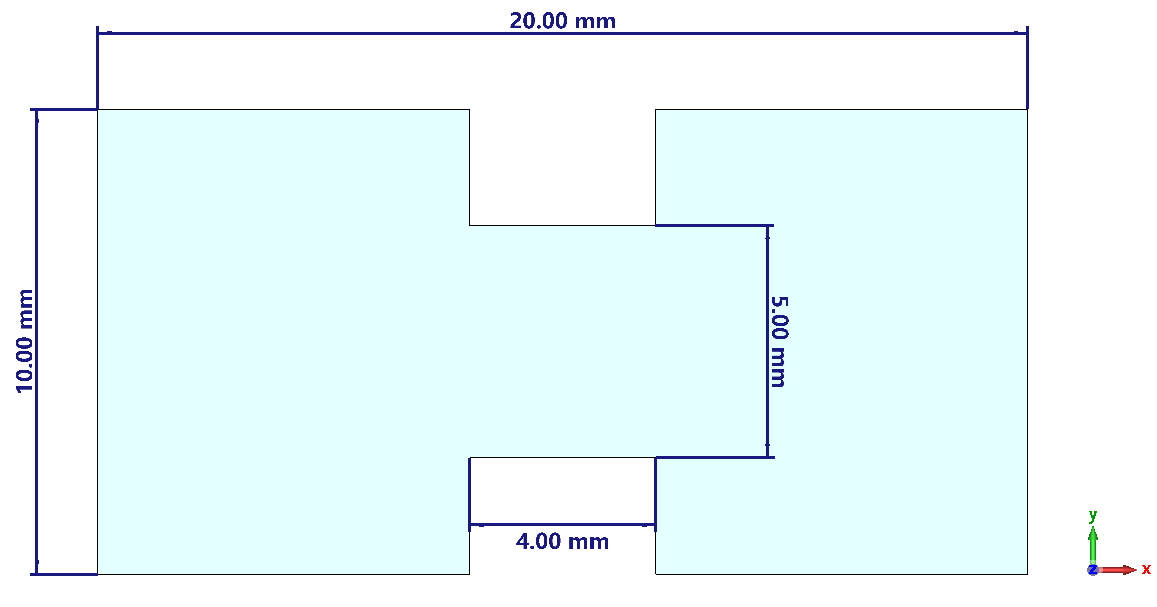
\includegraphics[width=0.7\linewidth]{pic/chapter3/6-11GHzDRW.png}
    \caption[short catption 1]{输入窗脊波导几何参数选取}
\end{figure}

很明显,这个脊波导的几何参数满足式子\ref{eq:DRW_constraints}的限制条件,此时可以通过简化式子\ref{eq:DRW_closed}计算双脊波导的截止频率进行计算,得到的计算结果为$f_c=5.85GHz$。此时截止频率小于所需带宽的下限,表明此时选取的脊波导几何参数满足要求。现在使用CST对脊波导的真实截止频率以及直通情况下的S参数进行仿真,得到如图\ref{fig:脊波导初步仿真}的结果。根据图\ref{fig:脊波导初步仿真} (a)结果显示,脊波导的截止频率为$f_c=5.84GHz$,与式子\ref{eq:DRW_closed}的计算结果基本一致。根据图\ref{fig:脊波导初步仿真} (b)显示,此时的双脊波导在要求的频段6-11GHz之内$S_{11}<25dB$,满足匹配要求。

\begin{figure}[!htb]
    \small
    \centering
    \begin{tabular}{@{\ }c@{\ }c}
        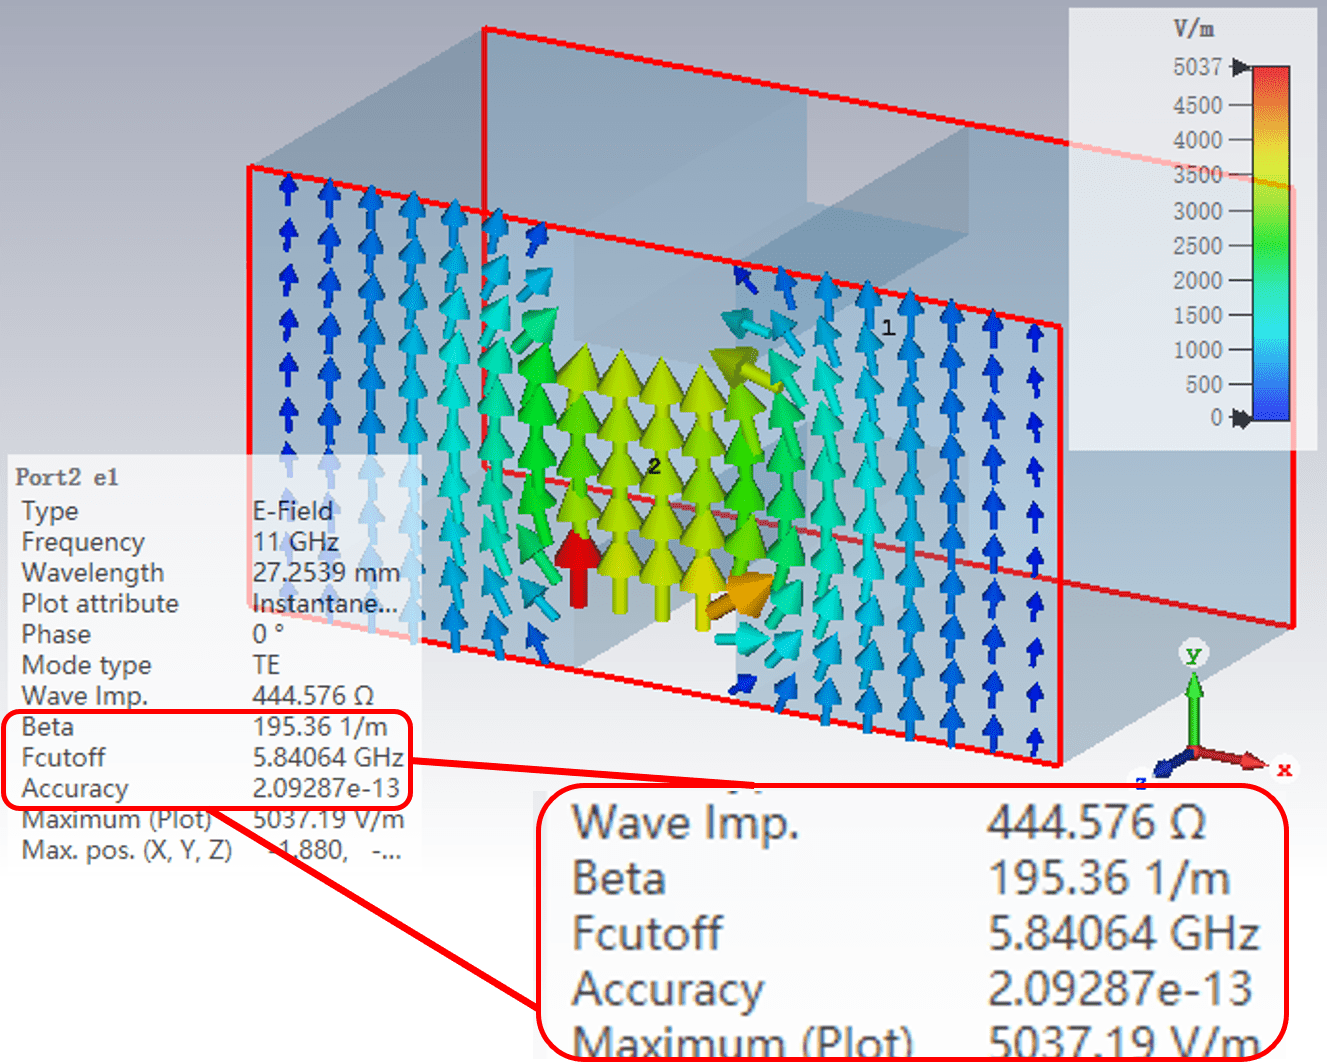
\includegraphics[width=0.45\textwidth]{pic/chapter3/脊波导初步仿真.png} & 
        \hspace{5pt}
        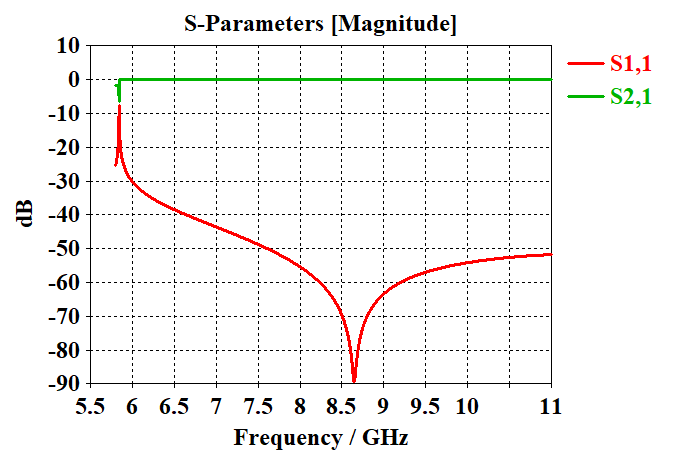
\includegraphics[width=0.45\textwidth]{pic/chapter3/输入窗脊波导S曲线.png}     \\
        \mbox{\small (a)脊波导截止频率仿真}                                                                               & 
        \mbox{\small (b)脊波导S曲线仿真}                                                                                  \\
    \end{tabular}
    \caption{脊波导初步仿真}
    \label{fig:脊波导初步仿真}
\end{figure}

接下来选取脊波导圆形窗片的材料,根据文章\cite{han_sapphire_2011}里面对窗片材料的论述,蓝宝石的特性包括低介电损耗和高机械强度,使其能够制造出0.1毫米厚的精细层而不会因为管内外压差而产生破损;由于它是致密无孔的晶体材料,内部结构均匀,所以在高功率操作环境下不易发生熔解破坏。此外,它还能应对焊接和真空脱气过程中的高温,当实现大规模生产时,成本控制良好,且环保方面的问题较少。因为蓝宝石的上述优点,本文选取蓝宝石作为窗片的材料。根据材料\cite{thumm_2020_State}所示,将蓝宝石的相对电介质常数设定为$\varepsilon_r=9.4$,损耗角正切被设定为$\tan \delta = 0.0004$。

经过计算仿真,最终确定脊波导窗片的整体结构为图\ref{fig:脊波导窗的整体结构}所示。
\begin{figure}[!htb]
    \centering
    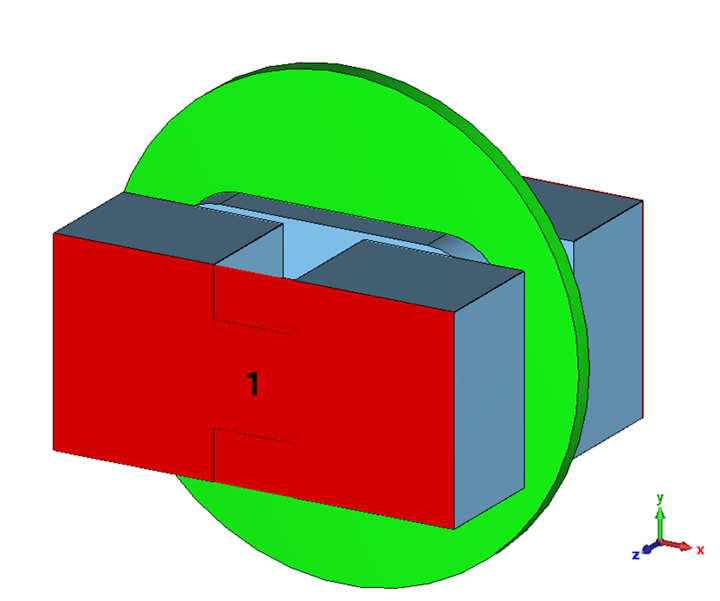
\includegraphics[width=0.45\linewidth]{pic/chapter3/输入窗的总体视图.png}
    \caption{脊波导窗的整体结构}
    \label{fig:脊波导窗的整体结构}
\end{figure}

为了方便设计加工与焊接,窗片被设置为圆形窗片。为了减少匹配段的长度,窗片与脊波导之间的过渡部分被设计为倒圆角的矩形过渡段。其中对过渡部分倒圆角不仅是为了降低过渡段的最大场强,提升窗片的功率容量,防止窗片被击穿;另一方面也方便了之后对过渡段部分的加工。

各个部分的详细尺寸被记载于图\ref{fig:窗片与过渡段的尺寸}中。其中\ref{fig:窗片与过渡段的尺寸} (a) 展示了窗片的直径为22.98mm。图片\ref{fig:窗片与过渡段的尺寸} (b)展示了圆窗片与脊波导之间的圆角矩形过渡段的具体尺寸,其长边为16.03mm,短边为10.61mm,四个角均倒圆角,倒圆角的半径为2.85mm。结构具体的纵向长度如图\ref{fig:窗片与过渡段的尺寸} (c)所示,圆角矩形过渡段的纵向长度为1.69mm,窗片的厚度为0.91mm。

\begin{figure}[!htbp]
    \small
    \centering
    \begin{tabular}{@{\ }c@{\ }c}
        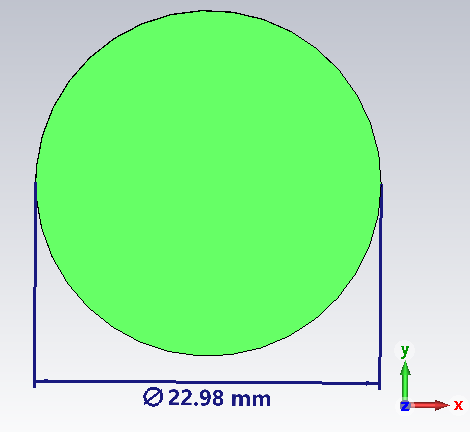
\includegraphics[width=0.25\textwidth]{pic/chapter3/圆形窗片视图.png} & 
        \hspace{5pt}
        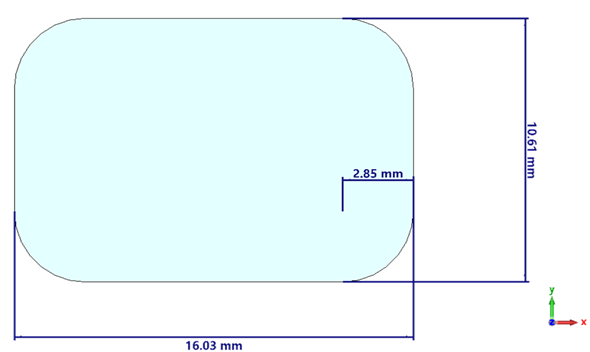
\includegraphics[width=0.45\textwidth]{pic/chapter3/圆角矩形视图.png}     \\
        \mbox{\small (a)圆形窗片视图}                                                                               & 
        \mbox{\small (b)圆角矩形视图}                                                                                  \\
    \end{tabular}
    \\[6bp]
    \begin{subfigure}[t]{0.75\linewidth}
        \setcounter{subfigure}{2}
        \centering
        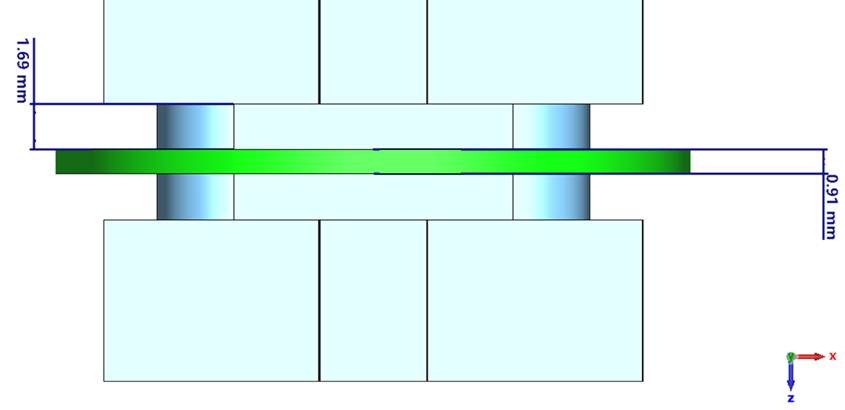
\includegraphics[scale=0.21]{pic/chapter3/纵向长度视图.png}
        \caption{纵向长度}
        \label{subfig:纵向长度视图}
    \end{subfigure}
    \caption{窗片与过渡段的尺寸}
    \label{fig:窗片与过渡段的尺寸}
\end{figure}


此时对脊波导窗的过渡段部分电长度进行分析,并与传统盒型窗进行对比。根据上文的分析,为了满足盒型窗窗片两侧过渡部分能够被等效为传输线的物理模型这一目的,传统盒型窗的匹配段部分不得小于0.1倍电长度。如果不满足这一要求就会因为无法被等效为传输线模型进而导致设计的匹配点出现频偏。此时新型盒型窗的过渡段可以被视作工作在$TE_{01}$下的长边为16.03mm,短边为10.61mm矩形波导,计算其在$10GHz$的工作波长为$\lambda_{gRec}=\lambda / \sqrt{1-(\lambda / \lambda_c)^2}=85.06mm$,匹配部分的电长度小于0.1倍电长度,相比于传统盒型窗的匹配部分的电长度更短,故新型窗片的匹配部分结构更加紧凑。

此时对原先参数的脊波导窗在CST里面进行建模,并且使用频域求解器在匹配频段内进行仿真,计算得到窗片的S参数如图\ref{fig:输入窗的S参数}所示:

\begin{figure}[!htb]
    \centering
    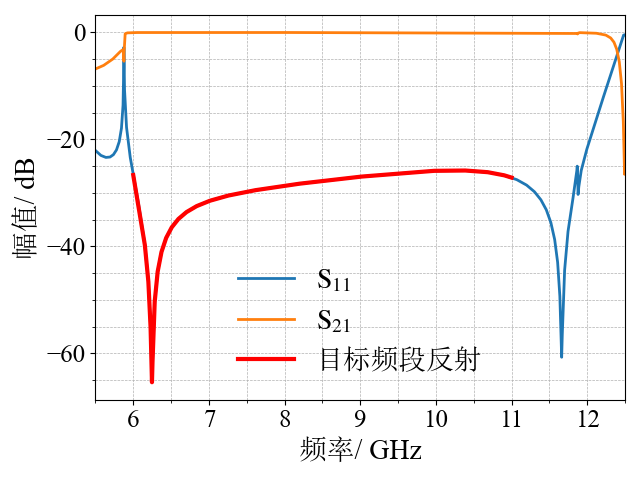
\includegraphics[width=0.5\linewidth]{pic/chapter3/脊波导窗S参数.png}
    \caption{输入窗的S参数}
    \label{fig:输入窗的S参数}
\end{figure}
对窗片的S参数进行考察,发现其反射系数$S_{11}$在要求的频段6-11GHz之内小于-20dB,满足匹配要求。此时结合图片可以得到满足反射系数$S_{11}<-20$的频带范围为6-11.5GHz,此时计算其相对带宽为62.9\%。
\section{脊波导窗的参数敏感度分析}
ERRORFIX。
\subsection{计算脊波导窗功率容量}
为了探究输入窗的适用范围,有必要对脊波导窗的功率容量进行分析。微波窗通常在电场强度最强处出现击穿,并且在扫参时候发现,在同一匹配频段内,低频点的电场强更强。根据之前的结论,现在对脊波导窗的在低频点处的电场场强进行仿真,得到如图\ref{fig:脊波导窗低频点场强仿真}所示的结果:
\begin{figure}[!htb]
    \centering
    
\includegraphics[width=0.25\linewidth]{pic/ERROR.jpg}
    \caption{脊波导窗6GHz场强仿真}
    \label{fig:脊波导窗低频点场强仿真}
\end{figure}

为了方便进一步地分析,需要找到最大电长场强所在位置,使用CST进行仿真之后可以得到其最大场强出现在ERROR,具体位置如\ref{fig:脊波导窗低频点场强仿真}所示:
\begin{figure}[!htb]
    \centering
    
\includegraphics[width=0.2\linewidth]{pic/ERROR.jpg}
    \caption{脊波导窗6GHz场强仿真}
    \label{fig:脊波导窗6GHz场强仿真}
\end{figure}

完成最大场强所在位置之后,可以开始对脊波导窗功率容量进行进一步的分析。为了确保结果的准确性,本文采用了两种不同的仿真方式进行对照。
\subsubsection{使用最大场强法计算脊波导窗的功率容量}
最大场强法主要是通过对端口的输入功率进行扫参,在最大场强达到30kV/cm的击穿场强时候被视为击穿,本文分析的最大场强值的参考主要来源于REFERROR,,,还没找到我去了都。但是在实际施行的过程中,窗片的实际功率容量并不全与这个方法所计算出来的功率容量相一致,实际的窗片的损毁原因是多种多样的,并不完全与最大场强相关。故在实际应用这个功率容量时候需要对仿真结果进行修正。

根据经验,在相同的馈入功率时候,低频点的最大场强值更大,本次仿真的频点就放在频段的低点(6GHz ) 处进行仿真。根据仿真结果\ref{fig:输入窗最大场强结果}显示,在馈入端口的功率到达7.5kW的时候,窗片内的最大场强达到30kV/cm。此时的窗片的功率容量应该在7.5kW左右。这个功率容量对于输入窗口来说已经足够。
\begin{figure}[!htb]
    \centering
    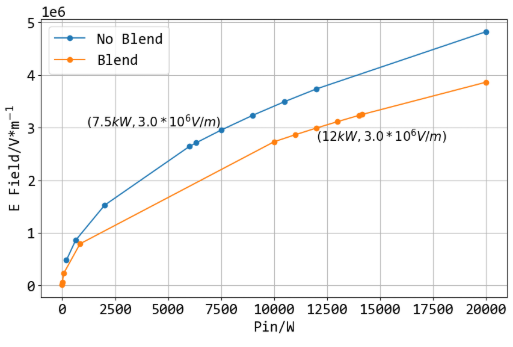
\includegraphics[width=0.5\linewidth]{pic/chapter3/脊波导最大场强.png}
    \caption{输入窗最大场强结果}
    \label{fig:输入窗最大场强结果}
\end{figure}
\subsubsection{使用二次电子发射计算脊波导窗的功率容量}
在太空之中,窗片结构中出现二次电子发射现象也是使得窗片发生损毁的重要原因之一。

\subsection{关于窗的多物理场分析}
为了验证窗片加工完成后的耐用性与稳定性,有必要对窗片的多物理场进行模拟分析。本次模拟仿真使用的软件为有限元仿真软件ANSYS,并且在模型外侧加装了一个铜制的金属外壳方便对加工完成后的情况进行模拟。
首先对窗片进行温度场分析,根据图片显示
根据经验,蓝宝石窗片在经过加热之后会出现热胀冷缩的现象
\section{模式变换部分的设计}
根据之前\ref{fig:6-11GHzDRW}的脊波导几何参数可以看出,此时的脊波导并非公用的标准脊波导,没有标准的同轴转脊波导的模式转换器。如果想要进行进一步的脊波导窗的测试,有必要设计脊波导转同轴的模式转换器。此时结合实际的测试情况,由于之前已经有标准矩形波导转同轴的模式转换器,并且在需要带宽内满足反射系数$S_{11}<-25dB$的反射系数要求。故设计脊波导到标准矩形波导的模式转换器。根据查表显示,标准矩形波导WR112的参数为28.499*12.624mm。并且为了标准矩形波导到脊波导之间测试件的纵向长度足够短足够紧凑,本文选取的模式变换主要结构为阶梯过渡,而不是渐变过渡。


\section{输出窗的相关研究}

\subsection{计算脊波导窗功率容量}
\subsubsection{使用最大场强法计算脊波导窗的功率容量}
\subsubsection{使用二次电子发射计算脊波导窗的功率容量}
\subsection{关于窗的多物理场分析}
\subsubsection{窗片的温度场分析}
\subsubsection{窗片的应力分析}
\section{小结}
\chapter{L 波段宽频带脊波导窗的设计}
\section{频带搬移时候出现的问题分析}

\section{L 波段宽频带脊波导窗的结构设计}

\section{计算L波段脊波导窗功率容量}
\subsection{使用最大场强法计算脊波导窗的功率容量}
\subsection{使用二次电子发射计算脊波导窗的功率容量}
\section{关于L波段脊波导窗片的多物理场分析}
\subsection{窗片的温度场分析}
\subsection{窗片的应力分析}
\section{模式变换部分的设计}
\section{小结}
\chapter{窗片测试产生的误差分析}
\chapter{全文总结与展望}
\chapter{README图表与相关引用规范}

角标参考文献\citing{chen2001hao}测试,普通参考文献~\cite{clerc2010discrete}。

这是符号\gls{tree}\cite{liuxf2006}。

$\hat{H}, f(x)$, $\vec{V}$

$$\hat{H}$$

$\mathcal{C}_i$

这是缩略词\acrlong{lvm}的长引用,这是缩略词的短引用\acrshort{lvm}。

\begin{figure}[!htb]
    \includegraphics[width=0.5\linewidth]{pic/figure.pdf}
    \caption[short catption 1]{Test caption 1}
\end{figure}


\begin{figure}[!htb]
    \small
    \centering
    \begin{tabular}{@{\ }c@{\ }c}
        \includegraphics[width=0.49\textwidth]{pic/figure.pdf} & 
        \hspace{5pt}
        \includegraphics[width=0.49\textwidth]{pic/figure.pdf}     \\
        \mbox{\small (a)随便试试的超级长的标题}                                                                               & 
        \mbox{\small (b)随便试试的超级长的标题}                                                                                  \\
    \end{tabular}
    \caption{随便试试的超级长的标题-总}
    \label{fig:test}
\end{figure}

\begin{figure}[!htbp]
    \centering
    \begin{subfigure}[t]{0.35\linewidth}
        \centering
        \includegraphics[scale=0.25]{logo.pdf}
        \caption{Fig. 1}
        \label{fig:1-1}
    \end{subfigure}
    \begin{subfigure}[t]{0.35\linewidth}
        \centering
        \includegraphics[scale=0.25]{logo.pdf}
        \caption{Fig. 2}
        \label{fig:1-2}
    \end{subfigure}
    \\[6bp]
    \begin{subfigure}[t]{0.35\linewidth}
        \centering
        \includegraphics[scale=0.25]{logo.pdf}
        \caption{求实求真}
        \label{fig:1-3}
    \end{subfigure}
    \begin{subfigure}[t]{0.35\linewidth}
        \centering
        \includegraphics[scale=0.25]{logo.pdf}
        \caption{Fig. 4}
        \label{fig:1-4}
    \end{subfigure}
    \caption{Fig.}
    \label{fig:1}
\end{figure}
算法框:

\begin{algorithm}[H]\label{alg:1}
    \KwData{this text}
    \KwResult{how to write algorithm with \LaTeX2e}
    initialization\;
    \While{not at end of this document}{
        read current\;
        \eIf{understand}{
            go to next section\;
            current section becomes this one\;
        }{
            go back to the beginning of current section\;
        }
    }
    \caption{How to wirte an algorithm.}
\end{algorithm}

这是算法\algref{alg:1}。

\thesisacknowledgement

xxxx % 直接填写致谢内容,写法与正文一致

\thesisbibliography[large]{reference.bib} % 参考文献

\thesisappendix
\chapter{xxxx} % 直接填写附录内容,写法与正文一致

% 攻读学位期间成果(本科不添加),例如:
\begin{thesistheaccomplish}
    \section{学术论文}
    \bibitem{SGXDedup} \textbf{Ren, Yanjing} and Li, Jingwei and Yang, Zuoru and Lee, Patrick PC and Zhang, Xiaosong. Accelerating Encrypted Deduplication via SGX[C]. Proc.of USENIX ATC, 2021, 957-971. \textbf{CCF-A}
    \section{发明专利}
    \bibitem{CN111338572B} 李经纬, 杨祚儒, \textbf{任彦璟}, 李柏晴, 张小松. 一种可调节加密重复数据删除方法:CN111338572B[P]. 2021-09-14.
\end{thesistheaccomplish}

% 以下为本科同学专用,插入文献翻译
\thesistranslationoriginal
\section{Tahoe-LAFS: The Least-Authority File System}
% \insertPDFPage{} % 用于插入单页PDF文件,例如原始文献(该操作会导致页码被取消,请谨慎使用)

\thesistranslationchinese
\section{Tahoe-LAFS:最小权限文件系统}

\end{document}
